\chapter{Systematic Uncertainty}\label{sec:systematic-uncertainty}
In this chapter, the systematic errors of the analysis are discussed. These uncertainties arise due to various reasons, some of them being the difference between real and simulated data, or due to the nature of the approaches taken in a specific analysis. Depending on their type, some uncertainties are generic and prepared beforehand in order to be used in all analyses, while others are analysis specific and possible sources need to be thought through thoroughly. All systematic uncertainties contributions which are cited in the final result in Section \ref{sec:branching-ratio-calculation-for-signal-decay} are summarized at the end of this chapter.

\section{Contributions to the Systematic Uncertainty}

\subsection{PID Efficiency Correction}\label{sec:pid-efficiency-correction}

The PID selection efficiency for the three charged particles in our signal decay needs to be corrected on MC due to various differences when comparing to data. The Belle PID group has prepared correction factors and a tables of systematic uncertainties for PID efficiencies for all charged particles. In case of kaon ID and lepton ID, the tables are binned in experiment numbers, particle momentum and in $\cos\theta$ of the particle direction, where, for each bin, a ratio of efficiencies between MC and data is provided, as well as the systematic errors. Each particle's correction factor and error is shown in Table \ref{tab:PID}, as well as the corresponding entry for all 3 particles. The entries are shown for both signal and control region, where the differences are related to the kinematic variations between the signal and control modes.

The central values were obtained with a weighted average over all experiments, where $100\%$ correlation for error calculation was assumed. A full correlation was also assumed when calculating the $KK$ correction, as both $K$ use the same PID information.

The final PID efficiency systematic error on the full MC sample is determined to be
\begin{equation}
\sigma_{\mathrm{sys}}^{\mathrm{PID}} = 10,\quad \delta_{\mathrm{sys}}^{\mathrm{PID}} = 2.0\%,
\end{equation}
for the signal as well as the control decay.

\begin{table}[H]
	\centering
	\begin{tabular}{l|c|c}
		PID correction and systematic uncertainties & Control decay & Signal decay \\
		\toprule
		Same sign $K$ (w.r.t the $B$ meson) & $1.005\pm 0.009$ & $1.007\pm 0.010$\\
		Opposite sign $K$ (w.r.t the $B$ meson) & $1.004\pm 0.009$ & $1.006\pm 0.009$\\
		$e$ & $0.977\pm 0.011$ & $0.976\pm 0.011$\\
		$\mu$ & $0.985\pm 0.009$ & $0.980\pm 0.009$\\
		$\ell$ & $0.981\pm 0.007$ & $0.980\pm 0.007$\\
		\midrule
		$KKe$ & $0.986 \pm 0.021$ & $0.988\pm 0.022$\\
		$KK\mu$ & $0.994 \pm 0.020$ & $0.993\pm 0.021$\\
		\midrule
		$KK\ell$ & $0.991 \pm 0.019$ & $0.990\pm 0.020$\\
		\bottomrule
	\end{tabular}
	\captionsetup{width=0.8\linewidth}
	\caption{PID correction factors and systematic error for various charged particles and their combinations.}
	\label{tab:PID}
\end{table}

\subsection{Fit Bias and Binning Effects}
Signal and background templates in our analysis are not perfectly distinct from one another and may potentially cause some over- or underestimation of the signal fit yield. In order to study this problem, we estimate the bias from the binning study performed in Section \ref{sec:signal-mc-fit-results} as well as the linearity test toy MC study in Section \ref{sec:pseudo-experiment-linearity-test}. The two bias functions describe a bias in each direction and are approximated as
\begin{align}
f_{\mathrm{min}}(x) &= -7.25-1.12x - \sigma_{f_{\mathrm{min}}}(x), \\
\sigma_{f_{\mathrm{min}}}(x) &= \sqrt{0.050 x^2 - 0.175 x + 0.410}, \\
f_{\mathrm{max}}(N_b) &= 6.86 + \sigma_{f_{\mathrm{max}}}(N_b), \\
\sigma_{f_{\mathrm{max}}}(N_b) &= \sqrt{0.004N_b^2 - 0.113 N_b + 1.112}
\end{align}
where $x$ represents the signal yield fraction of the data fit and $N_b$ represents the binning choice of the fit. Values of $1\sigma$ intervals have been added to the bias functions in order to be more conservative. The extracted signal yield on data  with the fit setup of $N_b=19$ bins was determined to be $N_{sig} = 491$, which leads to $x = N_{sig} / N_{sig}^{MC} = 491 / 249 \approx 2$. The bias interval is therefore
\begin{equation}
\sigma_{\mathrm{sys}}^{\mathrm{bias}} = {}^{+7}_{-10},\quad \delta_{\mathrm{sys}}^{\mathrm{bias}} = {}^{+1.5\%}_{-2.0\%}.
\end{equation}

\subsection{Gaussian Constraints}
As mentioned in Section \ref{sec:final-results-from-data}, it is possible to estimate the size of the systematic error of the Gaussian constraints. By fixing the constraints to the nominal values, determined by the data fit, we obtain the pure statistical error, which can then be subtracted from the average fit error in order to determine the systematic uncertainty contribution due to using Gaussian constraints. Due to the nature of implementing smearing of the $\Delta E$ variable, there is some randomness involved in our fits, so we perform 500 fits for the fixed and non-fixed case in order to determine the uncertainties. The split errors are then
\begin{align}
\bar \sigma_{\mathrm{fit}} &= 86, \\
\bar \sigma_{\mathrm{stat}} &= 81, \\
\sigma_{\mathrm{sys}}^{GC} &= 26,\quad \delta_{\mathrm{sys}}^{GC} = 5.4\%,
\end{align}
where GC stands for the Gaussian constraints. We see that the constrained channels are very well defined and introduce a relatively small level of uncertainty.


\subsection{Fit Template Smearing and Offset}
The smearing and offset of the $\Delta E$ variable was discussed in Section \ref{sec:smearing-and-offset-parameters}, where we have estimated the central value of the parameters as well as their range in the $1\sigma$ confidence level. We have to perform a study of the effects of different smearing and offset parameter values on the final value of the signal yield. From Section \ref{sec:smearing-and-offset-parameters}, the parameter values are
\begin{itemize}
	\item Smearing: $40_{-17}^{+15}\e{MeV}$,
	\item Offset: $6_{-6}^{+4.6}\e{MeV}$.
\end{itemize}
Since the two parameters are largely uncorrelated, we are able to perform the study in the form of signal fits with four different combinations of parameters in the given range. For each parameter setting the Gaussian constraints are fixed and 500 fits are performed to obtain the following results
\begin{itemize}
	\item Set: [smearing, offset]: $[23\e{MeV},6\e{MeV}],\quad$ Result: $ \bar N {}_{sig} = 458 $,
	\item Set: [smearing, offset]: $[55\e{MeV},6\e{MeV}],\quad$ Result: $ \bar N {}_{sig} = 532 $,
	\item Set: [smearing, offset]: $[40\e{MeV},0\e{MeV}],\quad$ Result: $ \bar N {}_{sig} = 532 $,
	\item Set: [smearing, offset]: $[40\e{MeV},12.6\e{MeV}],\quad$ Result: $ \bar N {}_{sig} = 460 $,
\end{itemize}
which results in the following estimate of systematic uncertainties for smearing and offset parameters
\begin{align}
\sigma_{\mathrm{sys}}^{\mathrm{sm.}} = {}^{+41}_{-33},&\quad \delta_{\mathrm{sys}}^{\mathrm{sm.}} = {}^{+8.3\%}_{-6.7\%}, \\
\sigma_{\mathrm{sys}}^{\mathrm{off.}} = {}^{+41}_{-31},&\quad \delta_{\mathrm{sys}}^{\mathrm{off.}} = {}^{+8.4\%}_{-6.3\%}.
\end{align}

\subsection{Effects of a Finite MC sample}
The shape of signal and backgrounds templates in our analysis is fixed and only their normalization is considered as a floating parameter in the fit. Due to the finite size of the MC sample, the template shape introduces an additional source of uncertainty, as it may differ if produced in a separate, equal-sized MC sample. Since the bins in these 2D histogram templates are statistically independent, we take the content of each bin and vary the value according to the Poisson distribution. This procedure is repeated 500 times with Gaussian constraints fixed and with a fixed random seed for smearing in $\Delta E$. The width of the fit yield distribution is taken as the uncertainty estimate. Since the systematic effects of the Gaussian constraints are included in the obtained distribution, we appropriately discard them to evaluate this systematic contribution. The resulting finite MC sample contribution of the systematic uncertainty is
\begin{equation}
\sigma_{\mathrm{sys}}^{MC} = 26,\quad \delta_{\mathrm{sys}}^{MC} = 5.3\%.
\end{equation}


\subsection{MVA Selection Efficiencies}
Control sample fits allow us to check the behavior of the optimized MVA selection on MC as well as data and see if any of the MVA steps introduce a possible disagreement between the two. We compare control yields, their ratios, and ratios of selection efficiencies (double ratios). The following selection criteria scenarios are studied
\begin{itemize}
	\item[(a)] final selection before any MVA step,
	\item[(b)] (a) + $BDT_{q\bar q}$ cut,
	\item[(c)] (a) + $uBDT_{B\bar B}$ cut,
	\item[(d)] (a) + $BDT_{q\bar q} + uBDT_{B\bar B}$ cut (final selection).
\end{itemize}

The results for control fit yields, their ratios, and double ratios are shown in Figure \ref{fig:cs_fits}. The plot shows that the yield ratios and selection efficiency ratios are consistent with $1$. This means that data and MC are in agreement before as well as after applying the final selection. This is an important check since the behavior of our analysis on the control sample suggests that the final selection is not over-optimized to signal MC.

We estimate the systematic error due to the MVA selection steps as the standard deviation of double ratio entries around the nominal value for each step in the MVA selection, except for the final two values for $e$ and $\mu$ modes, since we are performing the inclusive lepton measurement. The systematic error estimate for this contribution is 
\begin{equation}
\sigma_{\mathrm{sys.}}^{\mathrm{MVA}} = 5,\quad\sigma_{\mathrm{sys.}}^{\mathrm{MVA}} = 1.0\%.
\end{equation}

\begin{figure}[H]
	\centering
	\captionsetup{width=0.8\linewidth}
	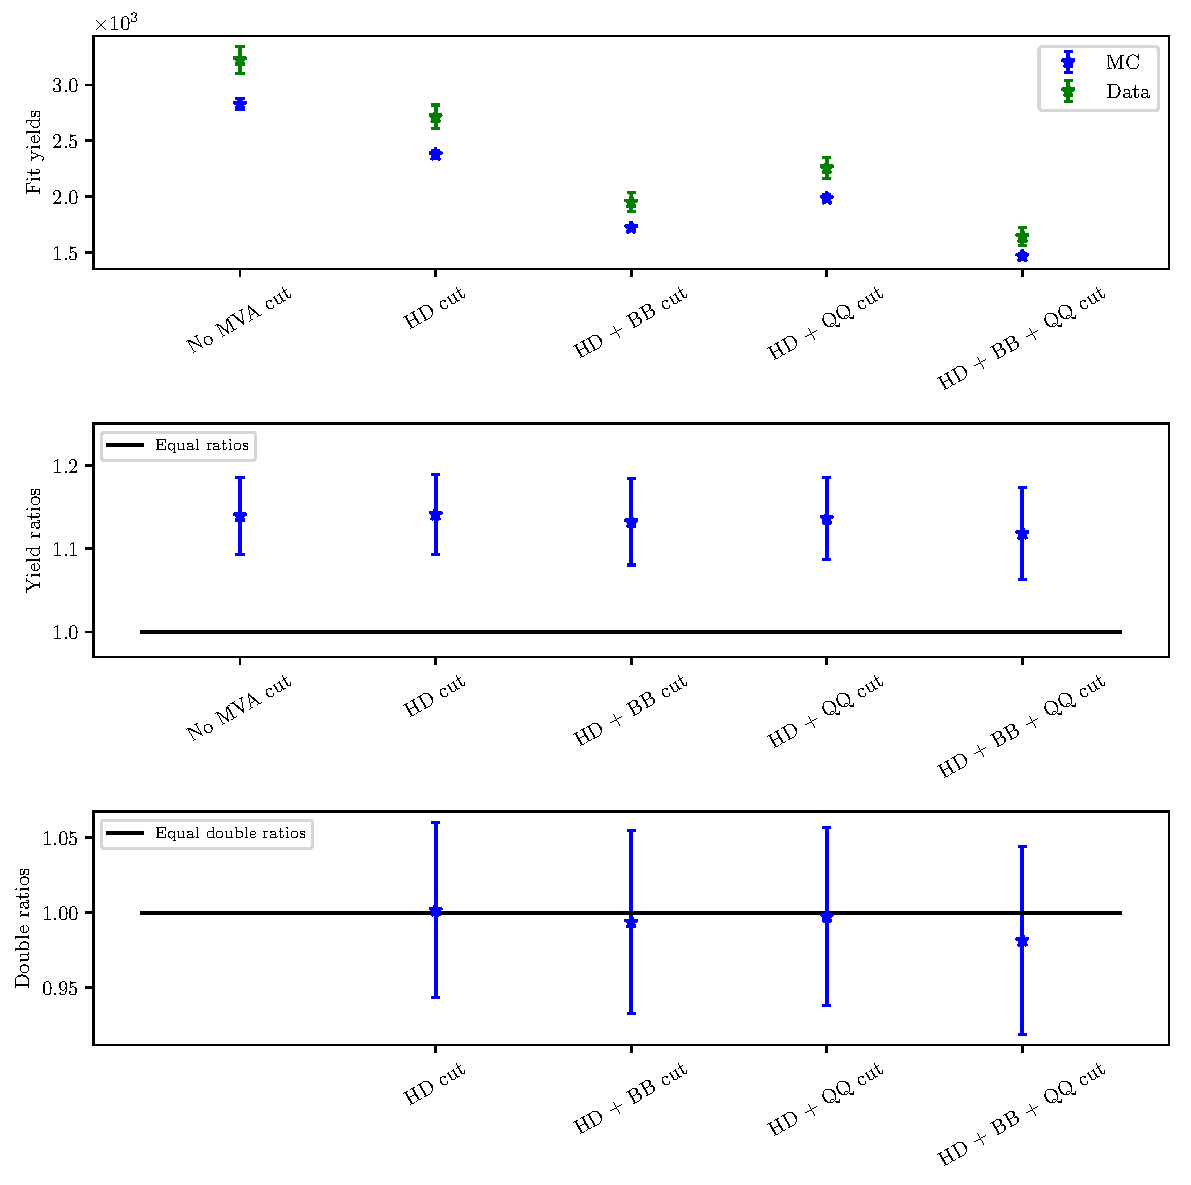
\includegraphics[width=\linewidth]{fig/cs_fits.pdf}
	\caption{Fit yields, their ratios and ratios of selection efficiencies (double ratios) for the control sample fits to data and MC.}
	\label{fig:cs_fits}
\end{figure}

\subsection{Model Uncertainty Effects}
The signal decay model used in the generation step is \texttt{ISGW2} \cite{Scora:1995ty}, which is known to result in unrealistic predictions and poor agreement with data, so it is not the most precise model for our signal MC sample. Due to this model unreliability, our analysis has been set up as model-independent as possible via means of not using variables, which exhibit model dependence. Such variables are squared momentum transfer to the lepton pair ($q^2$), the invariant mass of the two kaon daughters ($m_{KK}$) or decay angle between any two charged particles in the final state.
In order to test the effects of model dependency on our final result, we prepare three additional signal MC samples, produced with three extreme scenarios of decay model choice. In the first scenario we generate the signal MC sample with a generic phase-space decay mode \texttt{PHSP} \cite{lange2001evtgen}, which results in continuum-like distributions of $q^2$ and $m_{KK}$. In the other scenario, only resonant-like contributions of $m_{KK}$ are used. The third scenario is obtained by sampling the first model in a non-uniform way so that the final distribution is more dominant in the higher region of the $q^2$ distribution. These scenarios act as extreme cases of decay model choice and present a reasonable, if not a conservative measure of the model uncertainty. 

\subsubsection{Shape Effects of the Model}
The shape effect is evaluated by using signal templates, constructed from different signal MC samples. We perform 500 fits for each case with the Gaussian constraints fixed. The differences between mean values of fit yields serve as an estimate of the model uncertainty. Figure \ref{fig:model_cases} shows the generated $m_{KK}$ and $q^2$ distributions of the three mentioned decay models as well as distributions of \vars~after the final selection. Figures show a good agreement of \vars for different cases of the generator model.
\begin{figure}[H]
	\centering
	\captionsetup{width=0.8\linewidth}
	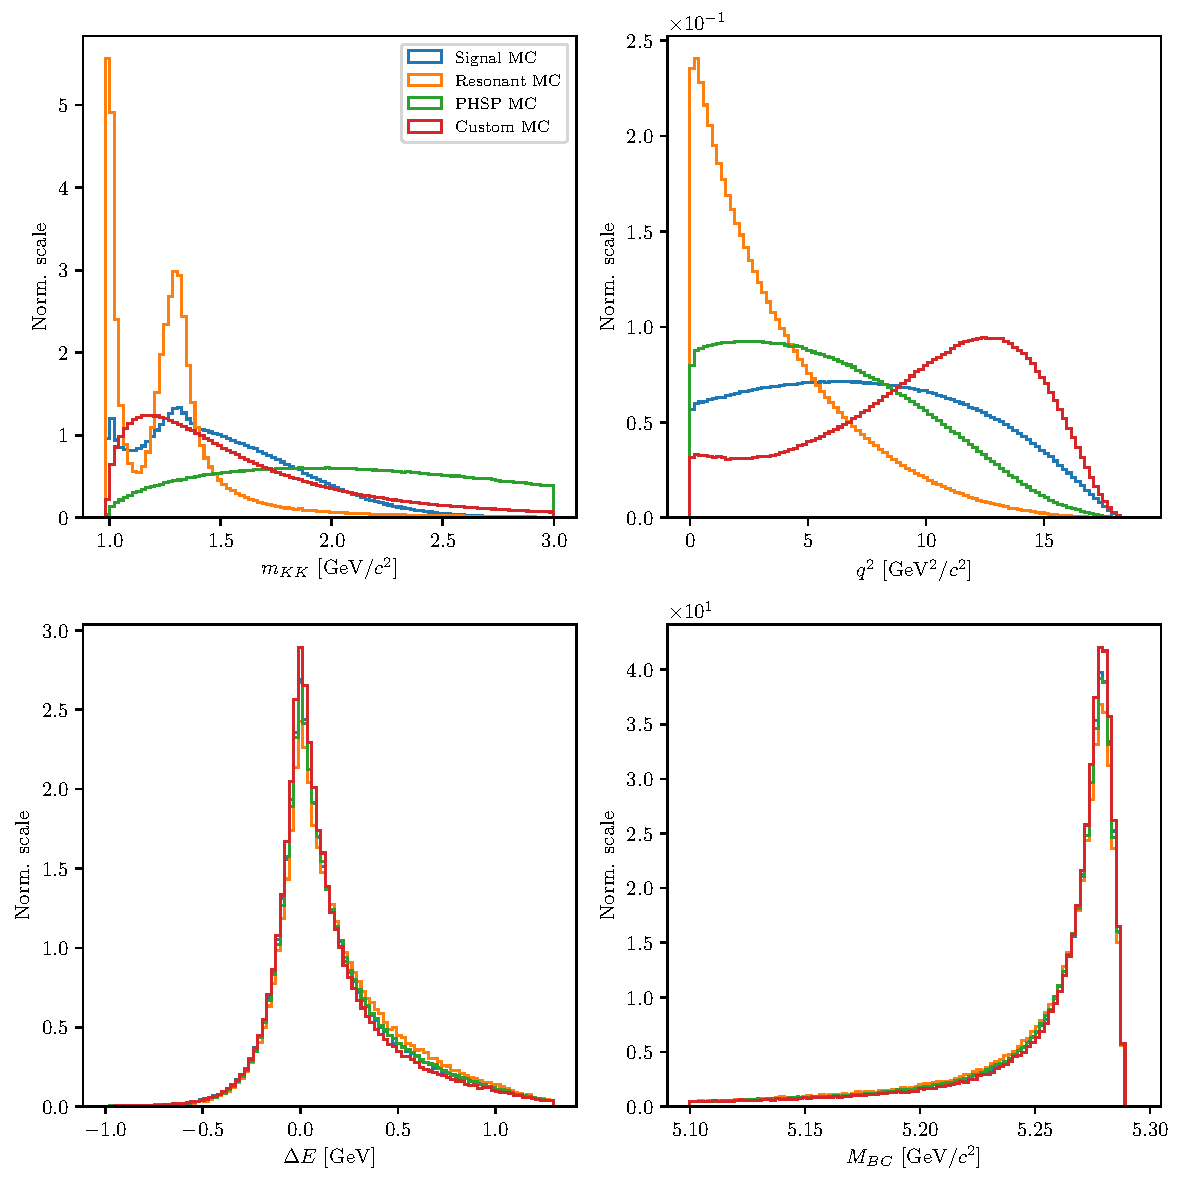
\includegraphics[width=\linewidth]{fig/model_cases}
	\caption{$m_{KK}$ (top left), $q^2$ (tip right), $\Delta E$ (bottom left) and $M_{BC}$ (bottom right) for the main and three extreme cases of signal MC generator choice.}
	\label{fig:model_cases}
\end{figure}
The resulting average signal yields for the three model choices are
\begin{align}
\bar N {}_{sig} &= 491, \\
\bar N {}_{sig}^{\mathrm{res.}} &= 494, \\
\bar N {}_{sig}^{\mathtt{PHSP}} &= 536, \\
\bar N {}_{sig}^{\mathtt{Custom}} &= 451.
\end{align}
We see that in general the model with a worse resolution in \vars~will likely result in a larger yield, and vice versa for a model with a better resolution. Overall these models give a conservative estimation of the systematic uncertainty due to the shape effects with a value of 
\begin{equation}
\sigma_{\mathrm{sys}}^{\mathrm{mod.}} = {}^{+45}_{-39},\quad \delta_{\mathrm{sys}}^{\mathrm{mod.}} = {}^{+9.3\%}_{-8.0\%}.
\end{equation}

\subsubsection{Model Efficiency}
The second way that the choice of a model can affect our analysis is the model efficiency. Due to the different properties of the model, we can expect different efficiencies in model dependent variables like $m_{KK}$ and $q^2$. The efficiency as a function of these variables is shown in Figure \ref{fig:efficiencies} for all discussed generator models. In a perfect scenario, a model-independent analysis should produce a flat efficiency as a function of the model dependent variables. While this is rarely achieved in practice, the overall discrepancy of the efficiency functions from very different models is relatively small.  
\begin{figure}[H]
	\centering
	\captionsetup{width=0.8\linewidth}
	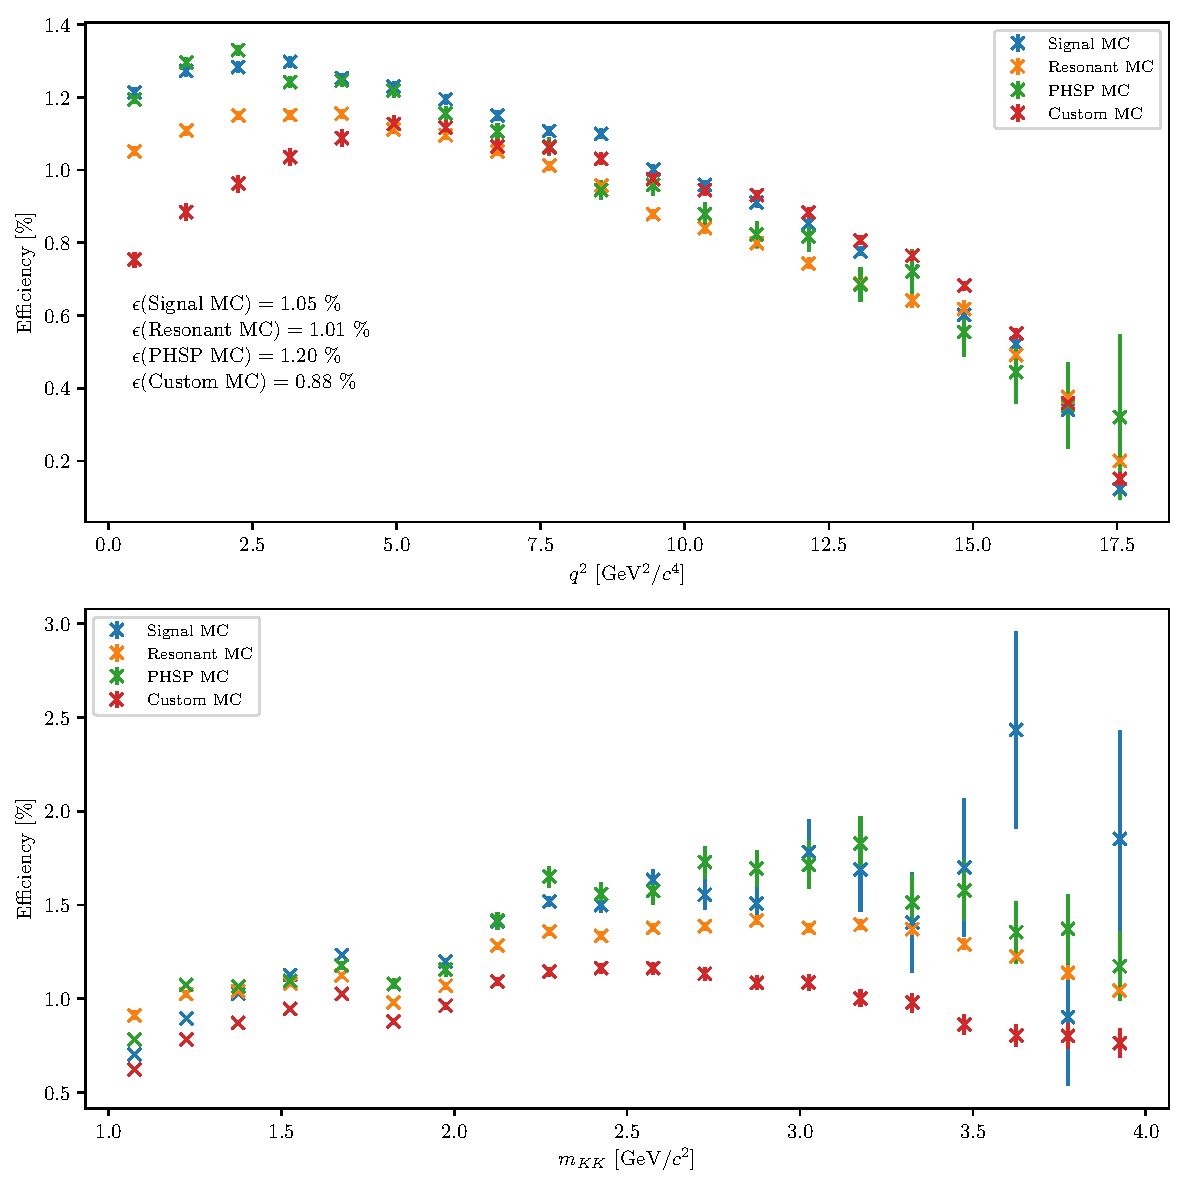
\includegraphics[width=\linewidth]{fig/efficiencies}
	\caption{Efficiency as a function of $q^2$ (top) and $m_{KK}$ (bottom) for the main and three extreme cases of signal MC generator choice.}
	\label{fig:efficiencies}
\end{figure}
To estimate the systematic uncertainty due to model efficiency effects, we compute the overall efficiencies and take the extreme cases of relative differences with regard to the main signal MC model. This results in
\begin{equation}
\sigma_{\mathrm{sys}}^{\mathrm{mod.}} = {}^{+70}_{-79},\quad \delta_{\mathrm{sys}}^{\mathrm{mod.}} = {}^{+14.3\%}_{-16.2\%}.
\end{equation}

As mentioned in Section \ref{sec:signal-distribution-in-bins-of-texorpdfstringq2q2}, measured $q^2$ and $m_{KK}$ distributions differ to some extent from the simulated ones. Since the reconstruction efficiency is not constant as a function of these variables, this could represent an additional source of systematic uncertainty. However, in $m_{KK}$, the measured signal is concentrated in the region $m_{KK}<2\e{GeV}/c^2$, where the efficiency is relatively constant in this interval and within the range of already estimated systematic uncertainty of around $\pm15\%$. In $q^2$, the data distribution is wider and encompasses the region of a more pronounced efficiency dependence. We estimated the branching ratio using the signal yield as obtained in bins of $q^2$ (see Table \ref{tab:q2_windows}) and the efficiency as a function of $q^2$. The result, although with a larger statistical uncertainty, due to low statistics in $q^2$ bins, is within the assigned systematic uncertainty due to the model dependency, and therefore consistent with the branching ratio found using the average reconstruction efficiency.

\section{Summary of Systematic Uncertainties}

The summary of all systematic uncertainties is shown in Table \ref{tab:sys_summary}. The full estimate of the systematic uncertainty is summed up in quadrature and applied to the result in Section \ref{sec:branching-ratio-calculation-for-signal-decay}.


\begin{table}[H]
	\centering
	\begin{tabular}{l|l|l}
		Source & $\sigma$ & $\delta~[\%]$ \\
		\toprule
		PID & $10$ & $2.0$ \\
		Fit Bias & $ {}^{+7}_{-10}$ & ${}^{+1.5}_{-2.0}$ \\
		Gaussian Constraints & $26$ & $5.4$ \\
		Template Smearing & ${}^{+41}_{-33}$ & ${}^{+8.3}_{-6.7}$ \\
		Template Offset & ${}^{+41}_{-31}$ & ${}^{+8.4}_{-6.3}$ \\
		Finite MC Effects & $26$ & $5.3$ \\
		MVA Selection & $5$ & $1.0$\\
		Model Shape & ${}^{+45}_{-39}$ & ${}^{+9.3}_{-8.0}$ \\
		Model Efficiency & ${}^{+70}_{-79}$ & ${}^{+14.3}_{-16.2}$ \\
		\midrule
		Total & ${} ^{+109}_{-107}$ & ${}^{+22.2}_{-21.9}$ \\
		\bottomrule
	\end{tabular}
	\captionsetup{width=0.8\linewidth}
	\caption{Summary of systematic uncertainties in this analysis.}
	\label{tab:sys_summary}
\end{table}







